\section{Implementation}

\begin{figure}
\centering
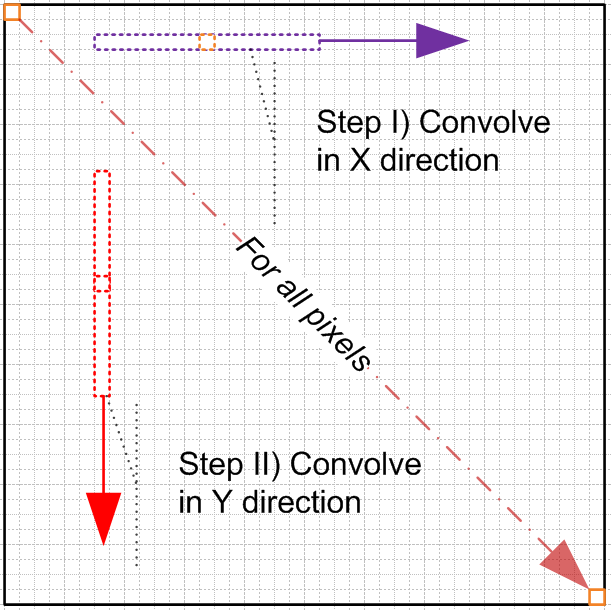
\includegraphics[width=0.4\textwidth]{drawings/gaussian_general}
\caption{Convolution process}
\label{fig:convolution}
\end{figure}

Obtaining the results from profiling we see that approximately 80\% of the time is spent on executing the \textit{gaussian\_smooth} function. Observing the code of this function we see that it is divided into two for loops (also seen in profiling output in figure~\ref{fig:prof}).
First the blurring is done by convolution in the X-direction and then in the Y-direction by applying the gaussian kernel (one dimensional convolution matrix). This process is briefly shown in figure~\ref{fig:convolution}. There is a data dependency between the two convolution processes where one must be followed by the other, so simply performing one convolution in one direction on one processing unit and the other direction on a different processor will not work.


\begin{figure}
\centering
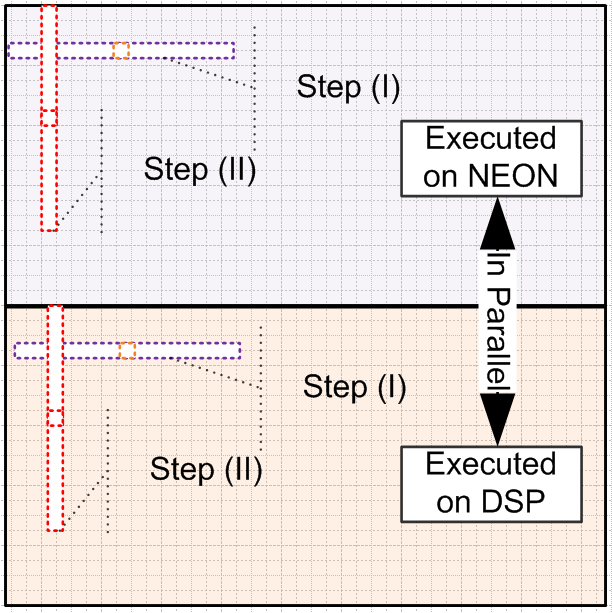
\includegraphics[width=0.4\textwidth]{drawings/gaussian_balancing}
\caption{Splitting the work}
\label{fig:balancing}
\end{figure}


The most naive way of splitting the work between two processors and obtaining a speed-up is to compute the gaussian filtering on both processors for different parts of the image. The most simplistic way with a 50/50 load balancing is depicted in figure~\ref{fig:balancing} where the NEON is performing the convolutions on the top part of the image and the DSP performs the convolutions on the bottom part of the image. As shown in the workflow diagram in figure~\ref{fig:workflow} we then proceed with the development of the gaussian filtering independently on each processor and later use clever techniques to split the computation between the two processors.


\begin{figure}
\centering
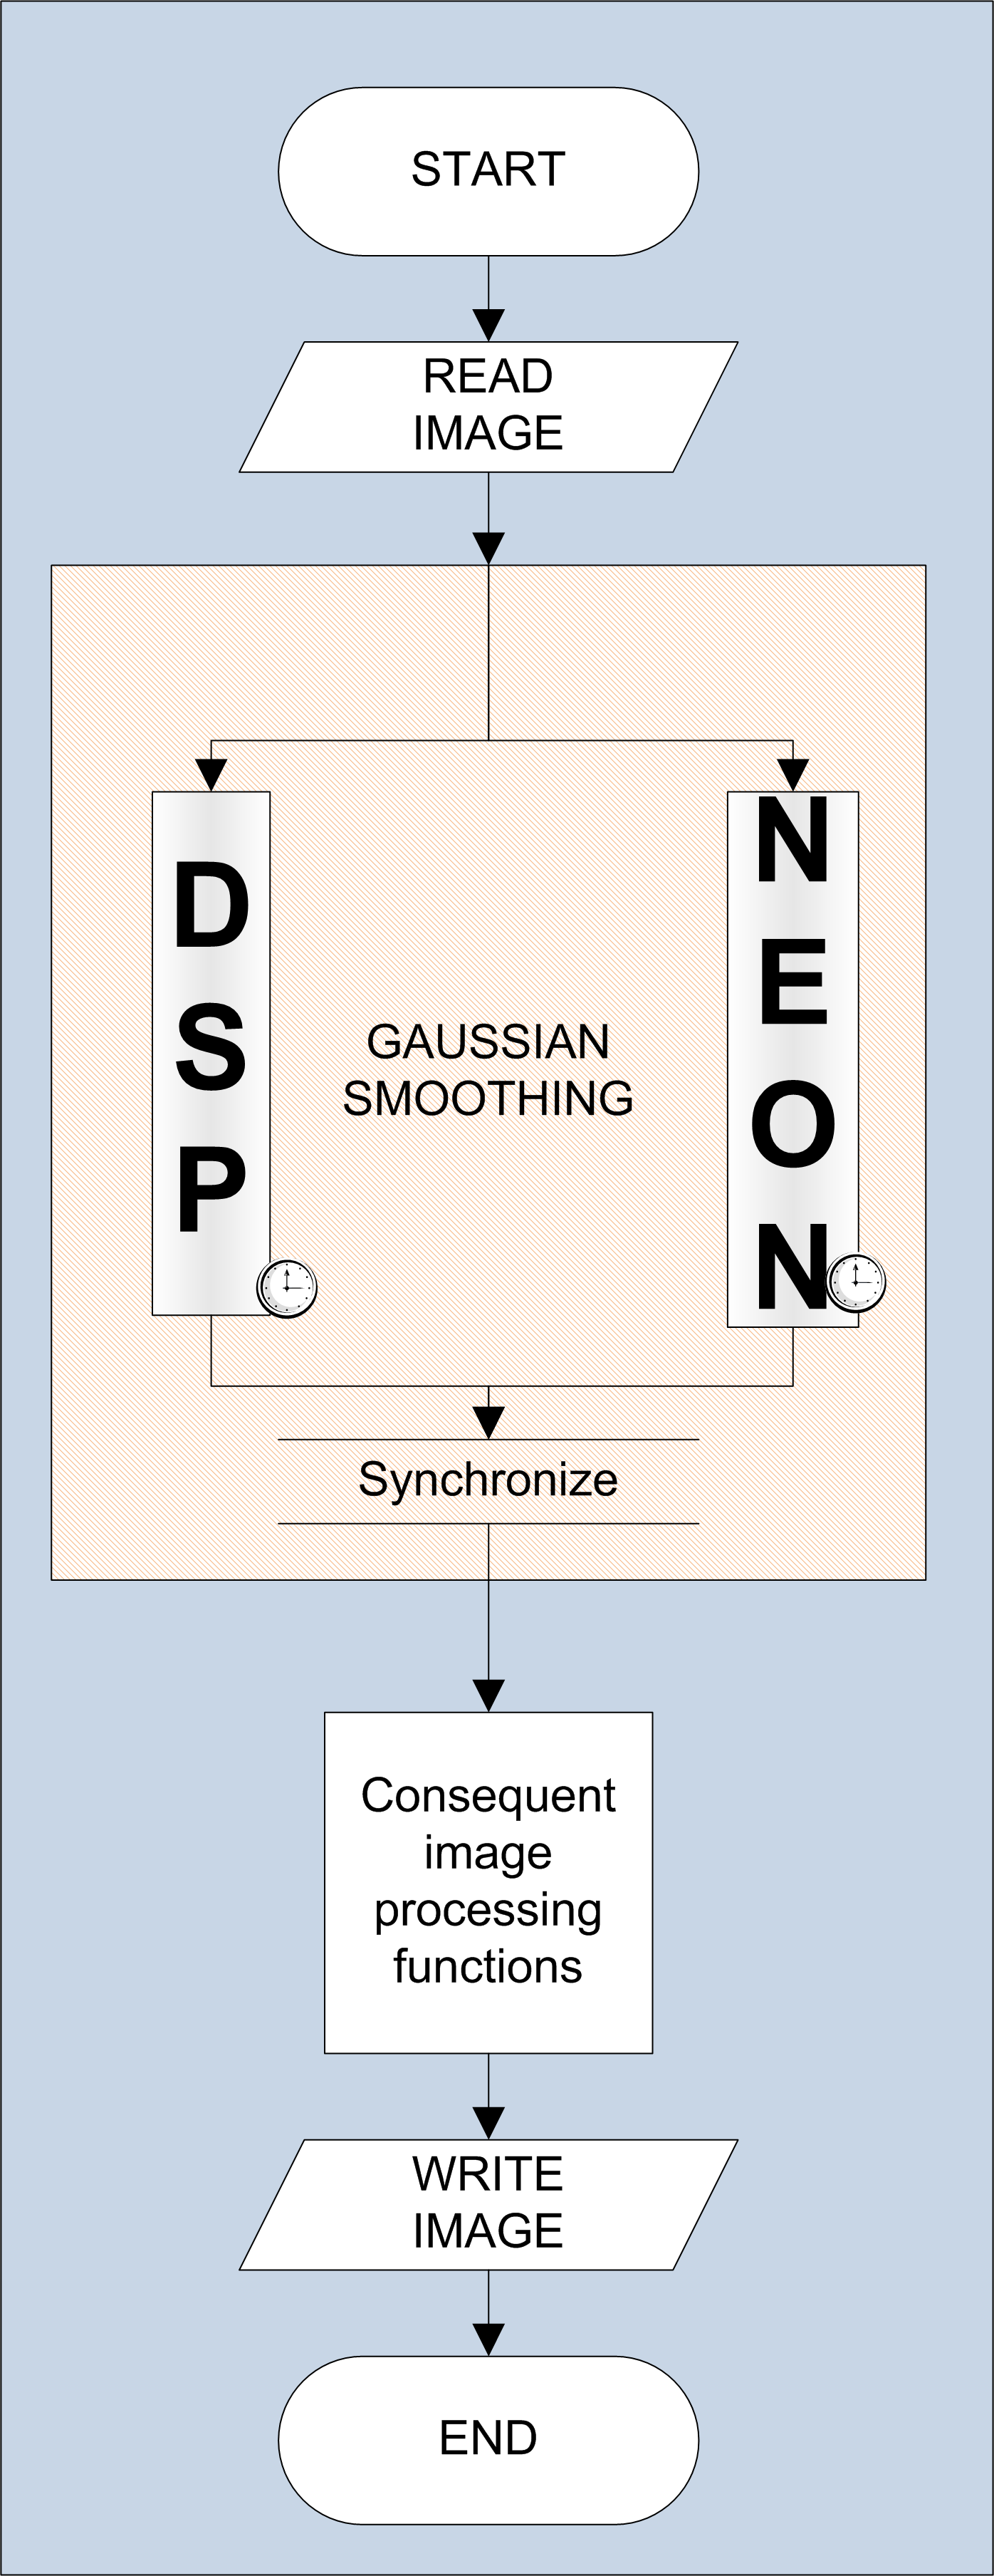
\includegraphics[width=0.25\textwidth]{drawings/model}
\caption{Data flow}
\label{fig:dataflow}
\end{figure}


On the gpp side we define FRAC which is an integer value from zero to hundred that specifies the fraction of calculations that must be done on the NEON. After integrating both compute units and making them work in parallel, both instances of gaussian smoothing calculations were measured in time and a FRAC that resulted in an even balance between gpp and dsp was chosen. Note that the two calculations have to be completed before the program can resume.
Hence, by load balancing we make sure that the synchronization happens as soon as possible and very little time is wasted on waiting for the slower processor to finish. Figure~\ref{fig:dataflow} shows the resulting dataflow of the current implementation. The subsequent sections go into more details of this process.


\section{DSP}
The \emph{OMAP3530} general purpose processor (from now on referred to as the
\emph{GPP}) contains a \emph{TMS320} digital signal processor (\emph{DSP}). This
core is optimised for using multiple calculation channels simultaneously: it is
a \emph{VLIW} (Very Long Instruction Word) processor that can utilise eight
functional units at the same time. More specifically, we can use six ALUs and
two multipliers per instruction. Another interesting feature is that each
multiplier can perform two 16 x 16-bit multiplications as well, giving us
potentially four multiplications in parallel.

The GPP unit is responsible for starting up the DSP core, giving it an executable to run
and afterwards detaching the core. Furthermore, the requirements specified
that the matrices to multiply are generated on the GPP core (which is 
of course not a bad idea because the GPP is way more flexible: it can easily
be changed to read the matrices from a file or standard input, and we can
offload a part of the work to the GPP itself and also the \emph{NEON} as we 
will discuss later as well). 

\subsection{Communication}
This however brings us to one complication: the matrices have to be moved to
the DSP core, while the (partial) end result has to be sent back to the GPP.
Our first goal is thus to set up communications and send matrices back and forth
between the two cores. 

\begin{figure}[h]
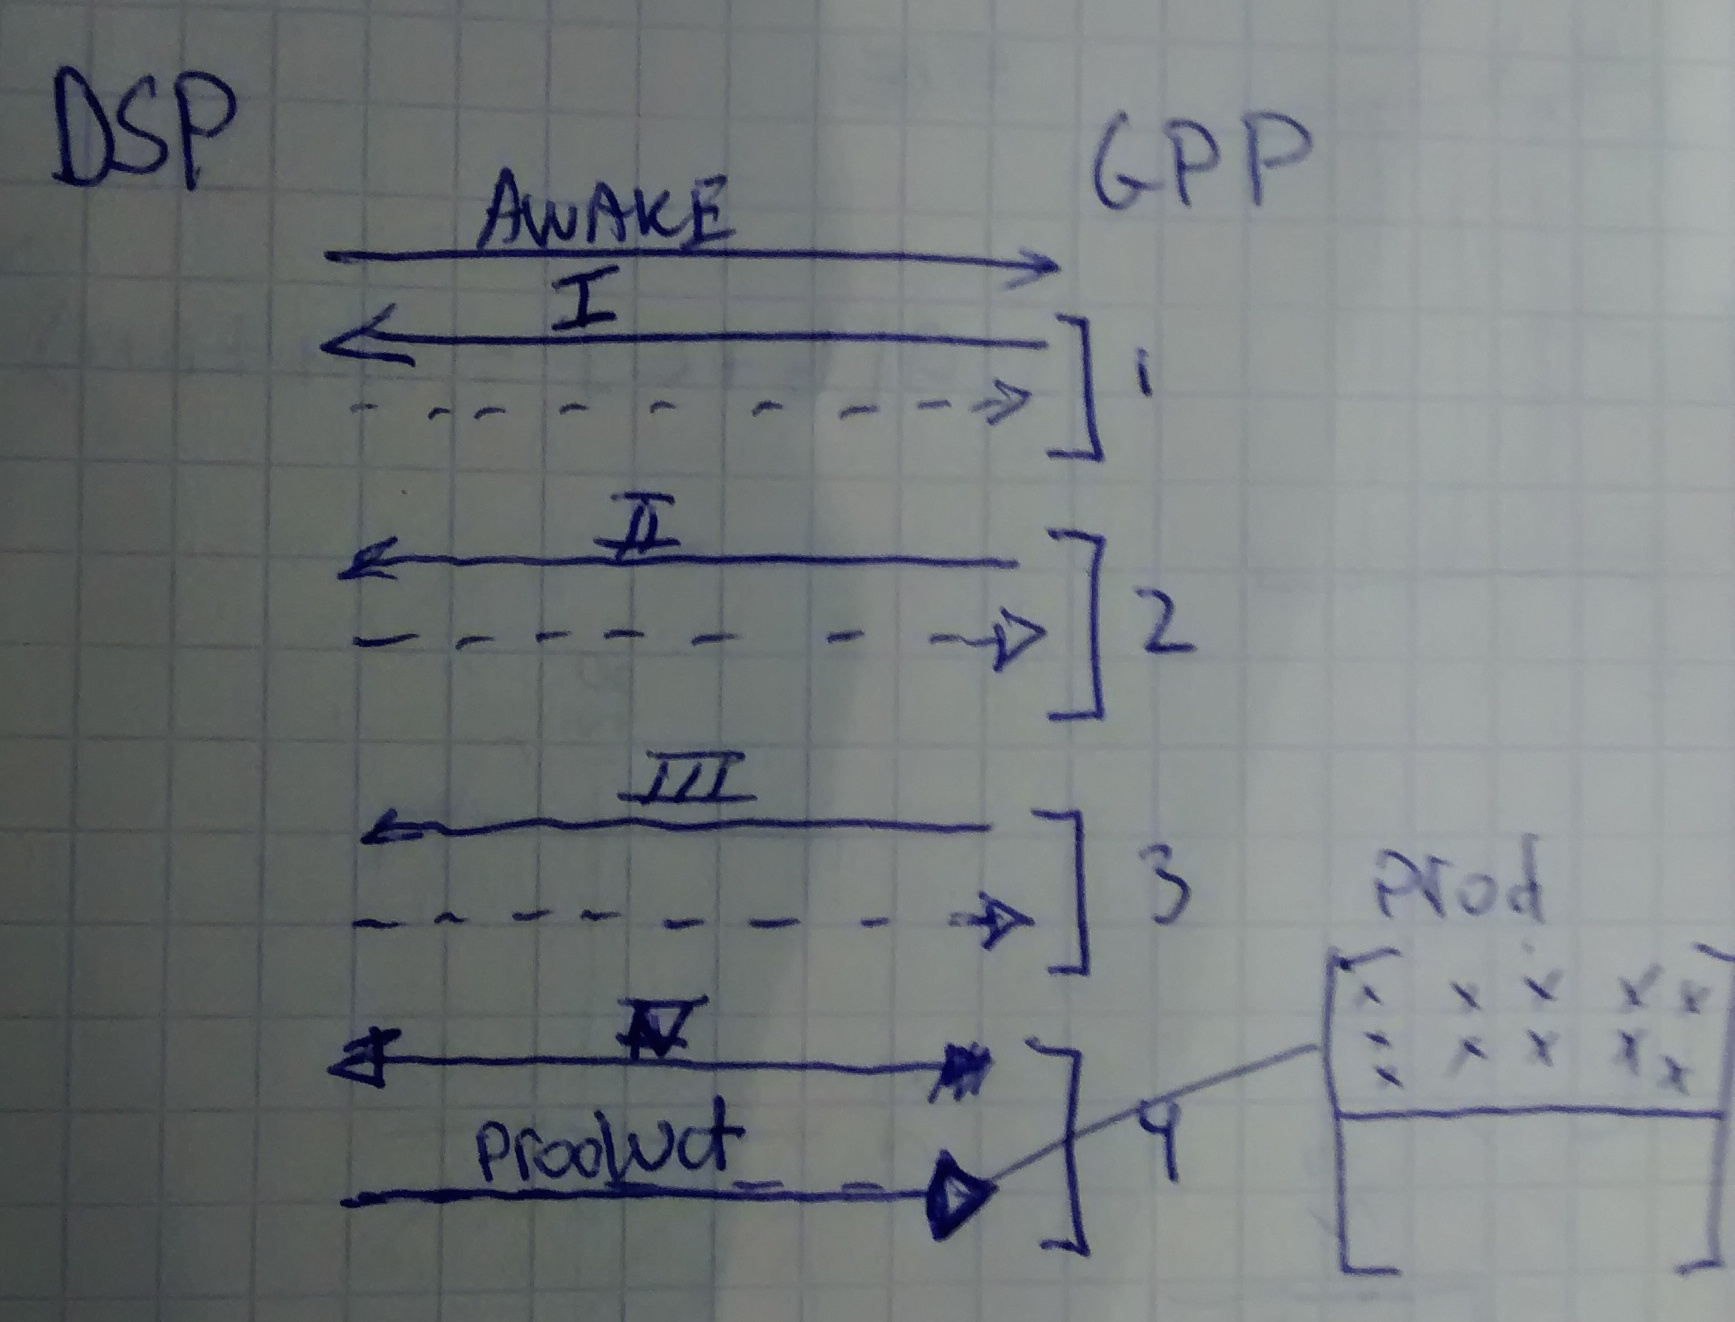
\includegraphics[width=\textwidth]{images/gpp_dsp_com}
\caption{Describing the communication process between the cores over time}
\label{fig:gpp_dsp_com}
\end{figure}

Unfortunately the communication API is slightly verbose and hard to handle.
For example, the sender has to allocate memory for a message, send it and the
receiver has the possibility to send it back, or free the message. If we opted
for the latter and re-allocate every message we would always crash the DSP core.
The former option would mean that if we wanted to send more than one message
directly from the GPP, the DSP would have to send the entire message back first.
We however observed that the communication overhead is negligible, so we
decided to always re-use the same message. The general communication time-line
is described in figure~\ref{fig:gpp_dsp_com}. One observation in this time-line
is that we send data six times. The reason why will be discussed in the next
section.

\subsubsection{Message Format}
We used the existing reference communication implementation and it's message
structure, but we extended it with our own matrices and an extra field that
indicates how big the resulting matrix should be. One thing we had to do 
was determine the maximum matrix size we could assign, such that it would fit 
in one message. This message would be stored inside a section of
\emph{APP\_BUFFER\_SIZE} large, thus our message structure has to fit in there. 
We experimentally found that we could send up to around 90k bytes per message.

The source matrices are 16 bit, but the result should be at least 32 bits. 
To accommodate for both 
situations in the same control message structure while optimally using our
message in a uniform way, we opted to use a \emph{union} structure so we 
can either send two 16 bit matrices or one 32 bit matrix at a time. The 
structure is given in figure~\ref{code:control_msg}. 

Because we have to send up to $128*128*2*2=65.536$ (2 matrices of 16 bits)
bytes from the GPP to the DSP, we need at least four messages considering
our bandwidth limit of 90k bytes. Thus we send the source in four messages, 
each containing a quarter of both matrices. The DSP only calculates a half of
the result matrix, making two messages sufficient: this results in six 
communication steps.

\begin{figure}[h]
\begin{lstlisting}[language=C]
struct mat2x16 {
	int16_t mat1[SIZE][SIZE];
	int16_t mat2[SIZE][SIZE];
};

struct mat32 {
	int32_t mat1[SIZE][SIZE];
};

typedef union {
	struct mat2x16 m16;
	struct mat32 m32;
} mat_t;

#define ARG_SIZE 256
typedef struct ControlMsg
{
    MSGQ_MsgHeader header;	// 20 bytes
    Uint16 command;				// 2 bytes
    Char arg1[ARG_SIZE];		// 256 bytes
    Uint8 size;					// 1 byte
    mat_t mat;						// 4 * SIZE * SIZE bytes
} ControlMsg;
\end{lstlisting}
\caption{The message structure we used}
\label{code:control_msg}
\end{figure}

\section{NEON}
To improve the performance of media and signal processing, 
\emph{NEON} SIMD technology is implemented in the \emph{Cortex-A8} core of the \emph{OMAP 3530} GPP. 
\emph{NEON} SIMD technology, which is also known as Advanced SIMD extension, 
takes the advantage of parallel operation to achieve the speed up.
\subsection{SIMD}
To understand NEON technology, the idea of SIMD is introduced at first. 
SIMD (Single Instruction Multiple Data) describes a way to perform the same operation on multiple data with same type and size in a single instruction. 
The idea of parallel operation comes from the fact that most of multimedia data are 16-bit or 8-bit wide, while the general purpose registers are 32-bit wide. 
To effectively utilize the space of registers, simultaneous computation is developed.  
\subsection{NEON Technology} 
\emph{NEON} technology, as the Advanced SIMD extension in \emph{Cortex-A8}, performs SIMD operations in group. 
NEON instructions operate on vectors stored in 64-bit or 128-bit registers, 
then vectors of elements with same type can perform the same operation on multiple items at the same time.
Figure~\ref{fig:neon} shows how multiple items are computed simultaneously. 

\begin{figure}[h]
\centering
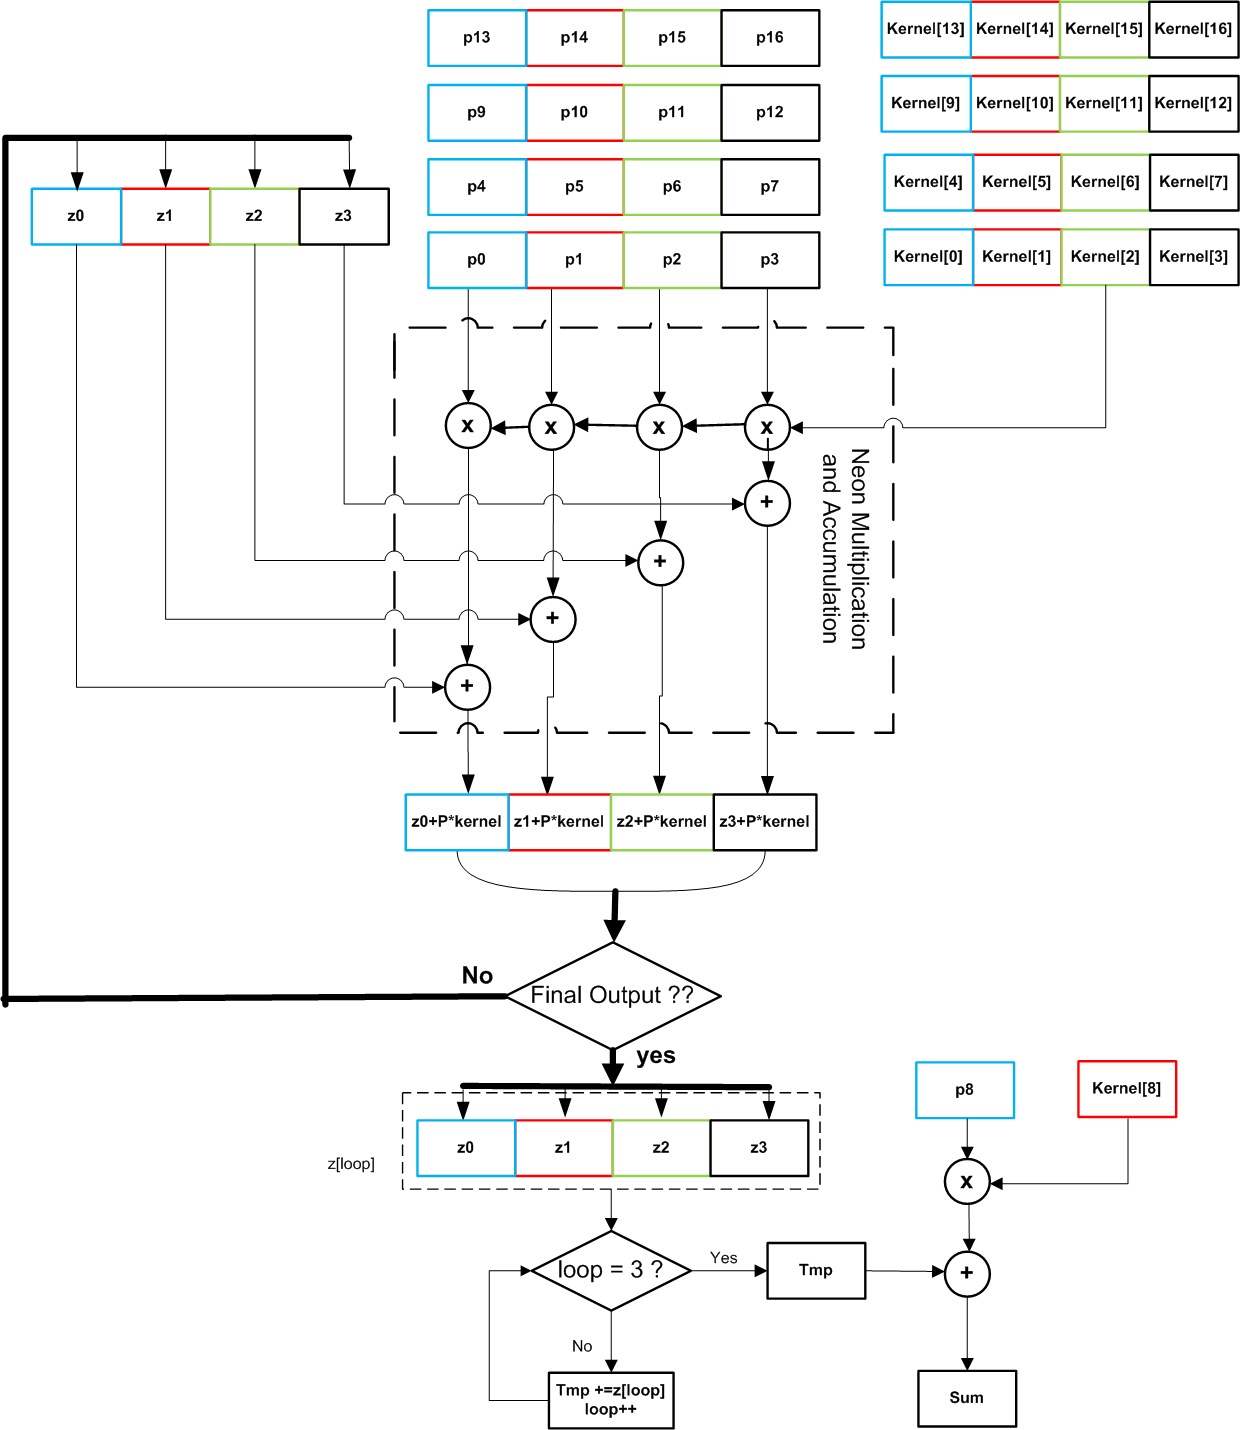
\includegraphics[width=0.9\textwidth]{images/neon}
\caption{Parallel computing based on NEON}
\label{fig:neon}
\end{figure}

\subsection{Hardware Features}
The NEON architecture has the following features\cite{hardware}:
\begin{enumerate}
\item \emph{16-Entry instruction queue}
\item \emph{32 x 64-bit general purpose registers in register file.}
These registers can alternatively be viewed as 16 x 128-bit registers
\item \emph{6-stage execution pipeline.}
NEON supports either integer or single precision floating point execute pipeline.
\item \emph{Load/store and permute pipeline}
\item \emph{12-Entry load data queue}
\end{enumerate}

\subsection{Implementation}
To enable the built-in intrinsics of NEON, 
\emph{$-$mfpu$=$neon}\cite{ARMoptions} is used during compiling time.
Also, the header file \emph{arm\_neon.h} is included 
to support NEON intrinsics in the c file.
In our case, the incoming message contains the matrix with data of 16-bit wide, 
and then after calculation, when the final outcome is sending back to GPP, the data size is 32-bit to avoid overflow.
In the following section, NEON intrinsics that are used for parallel computing in our experiment are explained.

\subsubsection{Vector Data Type}
Neon defined its own data type\cite{DataType} for multiple data operation, the format is given as:
~\\ 
\textbf{ \textless type\textgreater \textless size\textgreater x\textless number of lanes\textgreater\_t}

For example, the data type we are going to use in NEON is \emph{uint32x4\_t}, 
which means the vector has four lanes, 
with each of the them containing an unsigned 32-bit integer. 

\subsubsection{NEON Intrinsics}
NEON intrinsics \cite{Intrinsics} provide groups of functions for operation. 
In our case, functions related to load, multiplication and addition are used. 
\begin{enumerate}
\item \textbf{uint32x4\_t  vmovq\_n\_u32(uint32\_t value)}

This intrinsic loads all lanes of vector to the same input value. 
The input value is an unsigned 32-bit integer, 
while the four lanes being loaded each contains an unsigned 32-bit as well.


\item \textbf{int32x4\_t   vld1q\_s32(\_\_transfersize(4) int32\_t const * ptr)}

This intrinsic loads a single value from memory to all lanes.
The data stored in memory is signed 32-bit integer, 
while the four lanes each contains a signed 32-bit integer.

\item \textbf{int32x4\_t   vmlaq\_s32(int32x4\_t a, int32x4\_t b, int32x4\_t c)}

This intrinsic multiplies b by c, and accumulates the result with a in all four lanes.
The final results are then stored in four lanes as well.
\end{enumerate}

\subsubsection{Multiplication Algorithm}

In order to fully utilize the Neon resources, we have used following algorithm to compute the matrix multiplication. The following illustration shows one rows of results.
The input matrices are following:

$$
\begin{pmatrix}
 x1 	& \color{red}{x2} 	& \color{green}{x3} & \color{blue}{x4}\\
 x5 	& x6 				& x7&x8\\
 x9 	& x10 				& x11&x12\\
 x13 	& x14 				& x15&x16\\
\end{pmatrix}
\times
\begin{pmatrix}
y1&y2&y3&y4\\
y5&y6&y7&y8\\
y9&y10&y11&y12\\
y13&y14&y15&y16\\
\end{pmatrix}
$$


The output matrix would be : 
=
\begin{table}[h]
	\resizebox{\textwidth}{!}{
		$\left(
			\begin{tabular}{cccc}
				x1y1+\color{red}{x2}y5\color{black}{+}\color{green}{x3}y9\color{black}{+}\color{blue}{x4}y13&x1y2\color{black}{+}\color{red}{x2}y6\color{black}{+}\color{green}{x3}y10\color{black}{+}\color{blue}{x4}y14&x1y3\color{black}{+}\color{red}{x2}y7\color{black}{+}\color{green}{x3}y11\color{black}{+}\color{blue}{x4}y15&x1y4\color{black}{+}\color{red}{x2}y8\color{black}{+}\color{green}{x3}y12\color{black}{+}\color{blue}{x4}y16\\
				-&-&-&-\\-&-&-&-\\-&-&-&-\\
			\end{tabular}
		\right)$
	}
\end{table}

In the output matrix, the elements with the same color are multiplied by the Neon at the same time. In this way, Neon produces the results of 4 multiplications at the same time. In the output row above, x1y1, x1y2, x1y3 and x1y4 are produced by the neon simultaneously. However, these are just the partial results for the first row of output matrix. In order to get the complete results for the first row these partial results should be added to the other partial results of the same row. This complete task of multiplication and addition is done by using \emph{Multiplication and Addition} functional unit of neon. The conceptual diagram of this multiplication and addition is shown in figure~\ref{fig:neon_mult_add}.

\begin{figure}[h]
\centering 
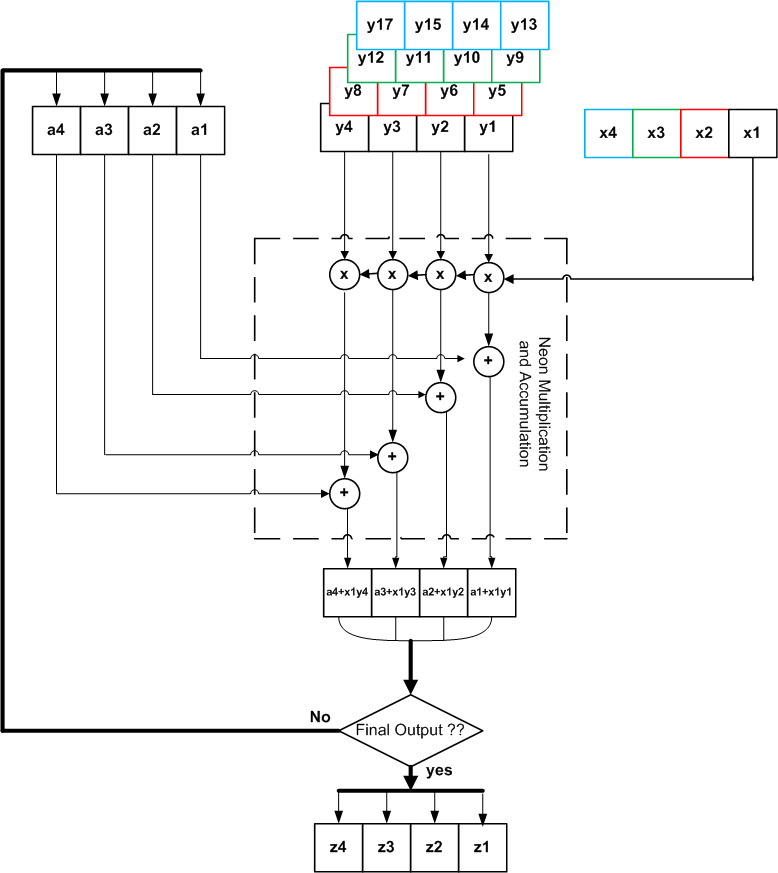
\includegraphics[width= 0.7\textwidth]{images/MandA}
\caption{Parallel Multiplication and Addition with Neon  }
\label{fig:neon_mult_add}
\end{figure}

